%%
%% Automatically generated file from DocOnce source
%% (https://github.com/hplgit/doconce/)
%%
% #ifdef PTEX2TEX_EXPLANATION
%%
%% The file follows the ptex2tex extended LaTeX format, see
%% ptex2tex: http://code.google.com/p/ptex2tex/
%%
%% Run
%%      ptex2tex myfile
%% or
%%      doconce ptex2tex myfile
%%
%% to turn myfile.p.tex into an ordinary LaTeX file myfile.tex.
%% (The ptex2tex program: http://code.google.com/p/ptex2tex)
%% Many preprocess options can be added to ptex2tex or doconce ptex2tex
%%
%%      ptex2tex -DMINTED myfile
%%      doconce ptex2tex myfile envir=minted
%%
%% ptex2tex will typeset code environments according to a global or local
%% .ptex2tex.cfg configure file. doconce ptex2tex will typeset code
%% according to options on the command line (just type doconce ptex2tex to
%% see examples). If doconce ptex2tex has envir=minted, it enables the
%% minted style without needing -DMINTED.
% #endif

% #define PREAMBLE

% #ifdef PREAMBLE
%-------------------- begin preamble ----------------------

\documentclass[%
twoside,                 % oneside: electronic viewing, twoside: printing
final,                   % or draft (marks overfull hboxes, figures with paths)
chapterprefix=true,      % "Chapter" word at beginning of each chapter
open=right               % start new chapters on odd-numbered pages
10pt]{book}

\listfiles               % print all files needed to compile this document

\usepackage{relsize,epsfig,makeidx,color,setspace,amsmath,amsfonts}
\usepackage[table]{xcolor}
\usepackage{bm,microtype}

\usepackage{ptex2tex}

\usepackage[T1]{fontenc}
%\usepackage[latin1]{inputenc}
\usepackage[utf8]{inputenc}

\usepackage{lmodern}         % Latin Modern fonts derived from Computer Modern

% Hyperlinks in PDF:
\definecolor{linkcolor}{rgb}{0,0,0.4}
\usepackage[%
    colorlinks=true,
    linkcolor=linkcolor,
    urlcolor=linkcolor,
    citecolor=black,
    filecolor=black,
    %filecolor=blue,
    pdfmenubar=true,
    pdftoolbar=true,
    bookmarksdepth=3   % Uncomment (and tweak) for PDF bookmarks with more levels than the TOC
            ]{hyperref}
%\hyperbaseurl{}   % hyperlinks are relative to this root

\setcounter{tocdepth}{2}  % number chapter, section, subsection

% Tricks for having figures close to where they are defined:
% 1. define less restrictive rules for where to put figures
\setcounter{topnumber}{2}
\setcounter{bottomnumber}{2}
\setcounter{totalnumber}{4}
\renewcommand{\topfraction}{0.85}
\renewcommand{\bottomfraction}{0.85}
\renewcommand{\textfraction}{0.15}
\renewcommand{\floatpagefraction}{0.7}
% 2. ensure all figures are flushed before next section
\usepackage[section]{placeins}
% 3. enable begin{figure}[H] (often leads to ugly pagebreaks)
%\usepackage{float}\restylefloat{figure}

% prevent orhpans and widows
\clubpenalty = 10000
\widowpenalty = 10000

% Make sure blank even-numbered pages before new chapters are
% totally blank with no header
\newcommand{\clearemptydoublepage}{\clearpage{\pagestyle{empty}\cleardoublepage}}
%\let\cleardoublepage\clearemptydoublepage % caused error in the toc

% --- end of standard preamble for documents ---


% insert custom LaTeX commands...

\raggedbottom
\makeindex

%-------------------- end preamble ----------------------

\begin{document}

% #endif


% ------------------- main content ----------------------



% ----------------- title -------------------------

\thispagestyle{empty}

\begin{center}
{\LARGE\bf
\begin{spacing}{1.25}
Epidemic models
\end{spacing}
}
\end{center}

% ----------------- author(s) -------------------------

\begin{center}
{\bf Torbjørn Seland${}^{}$} \\ [0mm]
\end{center}

    \begin{center}
% List of all institutions:
\end{center}

% ----------------- end author(s) -------------------------

\begin{center}
Dec 18, 2014
\end{center}

\vspace{1cm}


\newcommand{\Imax}{I_{\textrm{max}}}
\chapter{ODE models}
\label{section:ODE_models}
This chapter will be split into two different parts. The part includes two sections, which will be based on the chapter \emph{Dynamic of Infectious Diseases} from Mathematical Biology by J.D Murray Ref.\cite{murray2002mathematical}. \emph{Epidemic models} will give a historic perspective on different epidemic diseases and their effect on the human population. Furthermore a basic ODE system will be shown and studied to see how this model can give information about the disease. The section will check if a disease is severe for the human population, and based on this called an epidemic disease.


\vspace{3mm}




\vspace{3mm}


The last part will be based on a scenario where the population faces a zombification, one of the most critical and devastating epidemic diseases that can occur. Here, the TV series \emph{Walking Dead} will be used as reference, and the series will be tested against a model based on the SIR model explained in section \emph{Simple Epidemic models}. There have been a couple of papers on this model earlier, and this part will be based on these models and try to adjust the system to the TV series.     
\section{Simple Epidemic Models}
Most of the models shown here will have a constant population. The zombie model shown later will have a slight increase considering newborn, but this will be close to negligible. This may differ from the real world, where the population in different areas will vary with population flow. Reasons for doing this are, first of all to simplify the model and second to be able to model a closed system. How the population interacts is another assumption that has to be done. Here this is set to be similar for the whole area that is modeled. To simplify the population can be divided into three different groups. 
\begin{itemize}
\item \emph{Susceptible} ($S$), who are humans that are healthy and at risk of becoming infected. 

\item \emph{Infected} ($I$), who are humans who have the disease or are carriers of the disease. This group can infect the \emph{Susceptible}. 

\item \emph{Removed} ($R$),who are dead or recovering humans, often people that already have had the disease. 
\end{itemize}

\noindent
The natural order for a human is,
\begin{equation*}
S \rightarrow I \rightarrow R.
\end{equation*}
This model is called $SIR$ model, but the number of groups can be changed. $SI$ only consists of the two first groups and a $SEIR$ model has added an extra group \emph{Exposed} , $E$, where the disease is latent. This can be used to model the incubation time. 


\vspace{3mm}




\vspace{3mm}


The transmission of the infection and incubation period are elementary factors in the spread of a disease. These are reflected in the terms of the equations. Since this is a SIR model, the incubation time is negligible. The amount of people in each group can be seen as a function of time, expressed as $S(t),I(t)$ and $R(t)$. The growth of $I$ caused by \emph{Susceptible}, can be viewed as a rate proportional to the number of \emph{Infected} and \emph{Susceptible} multiplied by a constant,$rSI$, where $r>0$. This constant controls the efficiency of the transmission from $S$ to $I$. This will appear as a reduction in the function $S(t)$. The rate of removal from \emph{Infected} to \emph{Removed} can be viewed as the number of \emph{Infected} times a constant, $aI$, where $a>0$ controls the time spent in the \emph{Infected} group. The dynamic model will be,
\begin{equation} \label{eq:SIR_model}
	\begin{aligned} 
	\frac{dS}{dt} &= -rSI \\ 
	\frac{dI}{dt} &= rSI-aI \\ 
	\frac{dR}{dt} &= aI 
	\end{aligned}
\end{equation}
This model is called the Kermack-McKendrick(1927) model Ref.\cite[p.~320]{murray2002mathematical}.~It is considered that the groups are uniformly mixed and that there is equal probability of contact for all individuals. These assumptions will not be correct for all diseases, especially sexually transmitted diseases. The total number of the population will stay constant, since this is a closed system. This can be seen on the total change.
\begin{equation}
\frac{dS}{dt} + \frac{dI}{dt} + \frac{dR}{dt} = 0
\end{equation}

Therefore the total size of the population, $N$, will be constant. 
\begin{equation} \label{eq:SIR_N}
S(t)+I(t)+R(t) = N
\end{equation}

\section{Threshold phenomenon}
\label{section:1threshold_phenomenon}
The threshold value is essential when studying an epidemic model. To cause an epidemic situation, the model needs to fulfill $I(t)> I_0$ for some $t>0$, where $I_0$ describes the initial condition of  the \emph{Infected} group. The initial conditions can be given as,
\begin{equation} \label{eq:thres_val}
S(0)=S_0 > 0,\hspace{8mm} I(0)=I_0>0,\hspace{8mm} R(0) =0.
\end{equation}
These initial conditions given in Eq.(\ref{eq:thres_val}) combined with $r$ and $a$ controls the epidemic situation. These will affect the spread of the infection. From Eq.(\ref{eq:SIR_model}) the function for the \emph{Infected} group at initial time is,
\begin{equation}
\left[\frac{dI}{dt}\right]_{t=0} = I_0(rS_0-a)
\end{equation}
The expression inside the brackets controls the change in $I$. The function will increase if $S_0 > \frac{a}{r}$, this will therefore be the threshold value for the function. The threshold value will be described by the variable $\rho$,
\begin{equation} \label{eq:threshold_value}
\rho = \frac{a}{r}
\end{equation}
This can be shown with some phase trajectories of the \emph{Susceptible} and the \emph{Infected} in Fig.(\ref{fig:threshold_phenomenon}).  


\begin{figure}[ht]
  \centerline{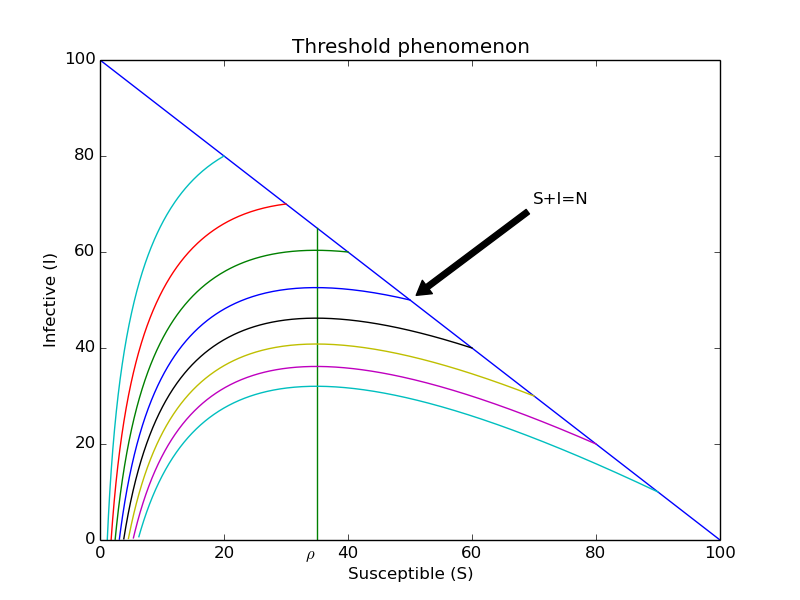
\includegraphics[width=0.8\linewidth]{1_fig/threshold_phenomenon.png}}
  \caption{
  \label{fig:threshold_phenomenon} Simulations of the SIR model (\ref{eq:SIR_model}) with start positions along the blue line. $I$ increases until $S$ is equal to the threshold value $\rho$, which is set to 35. Then $I$ is reduced to 0. In the simulations where $S_0 < \rho$, no epidemic situation is achieved.
  }
\end{figure}
%\clearpage % flush figures fig:threshold_phenomenon


The simulation shows that $I$ is based on the relation between $S$ and $\rho$. This can be described with a reproduction rate,
\begin{equation}
R_0 = \frac{rS_0}{a}
\end{equation}
It will cause an epidemic reaction if $R_0 > 1$. This parameter is crucial in the understanding of the work with the disease. To prevent a dispersion, the value of $R_0$ has to be under 1. An effective way to get control is by global vaccination programs. Smallpox is an example on a disease that nearly has been eradicated around the world. This is due to a reduction of \emph{Susceptible}. However there is always a small chance of side effects when using vaccination, and therefore some people choose to skip it. This is quite critical for the fight of total eradication. Not only is it a big risk for the specific person, but it also increases the number of \emph{Susceptible}. An epidemic situation can quickly grow again if the reproduction rate reaches the threshold.


\vspace{3mm}




\vspace{3mm}


Some analytical studies can be done on the model in Eq.(\ref{eq:SIR_model}).
\begin{equation} 
\frac{dI}{dS} = -\frac{(rS-a)I}{rSI} = -1 + \frac{\rho}{S},\hspace{8mm}\rho=\frac{a}{r}, (I\neq0).
\end{equation}
The singularities will all lie on the I=0 axis. This equation can be integrated and will then give phase plane trajectories in the (I,S) plane. This can be seen in Fig.(\ref{fig:threshold_phenomenon}).
\begin{equation} \label{eq:constant}
I+S-\rho \ln S = \textrm{constant} = I_0 + S_0 - \rho \ln S_0
\end{equation}
All initial values satisfy $I_0+S_0=N$ since $R(0) = 0$. This will change when $t>0$. If a disease appears it would be important to know the severity of the disease and the chance of developing to an epidemic disease. Therefore it is crucial to know the maximum value $\Imax$ which occurs when $S=\rho$. At this point, $\frac{dI}{dt}=0$. This can be found by using (\ref{eq:constant})
\begin{align} 
I+S-\rho \ln S =& I_0 + S_0 - \rho \ln S_0 \nonumber \\
\Imax+\rho-\rho \ln \rho =& I_0 + S_0 - \rho \ln S_0\nonumber \\
\Imax=&- \rho+\rho \ln \rho + I_0 + S_0 - \rho \ln S_0\nonumber \\
\Imax=&N - \rho + \rho \ln\frac{\rho}{S_0} \label{eq:max_I}
\end{align}
The different trajectories in Fig.(\ref{fig:threshold_phenomenon}) shows the difference between $S_0 > \rho$ and $S_0 < \rho$. An increasing of the \emph{Infected} group will occur in the cases where $S_0$ is higher. While a decreasing will happen when $S_0$ is lower. An example can be shown. The $\rho$ in the simulation in Fig.(\ref{fig:threshold_phenomenon}) is set to 35, while $N=100$ for all trajectories. A calculation can be done on the lowest trajectory which has the initial conditions $S_0= 90$ and $I_0= 10$
\begin{align*}
\Imax =& N-\rho + \rho \ln \frac{\rho}{S_0}\\
\Imax =& 100-35 + 35 \ln \frac{35}{90}\\
\Imax =& 31.94
\end{align*}
This situation causes an epidemic situation since $\Imax$ is much higher than the initial condition $I_0$. The Fig.(\ref{fig:threshold_phenomenon}) shows that the trajectory of this function starts decreasing after this point. In the two upper trajectories where $S_0 < \rho$, the \emph{Infected} group starts decreasing from the initial condition. The \emph{Infected} group will decrease towards zero as $t\rightarrow \infty$.

\section{English Boarding School 1978}
The British medical journal published a report from a boarding school in England in 1978. One of the boys had brought with him a disease back to the school. Since this was a boarding school, they were totally isolated from others and had a closed system to model \cite[p.~325]{murray2002mathematical}.~The simulation can be seen in Fig.(\ref{fig:english_boarding})  


\begin{figure}[ht]
  \centerline{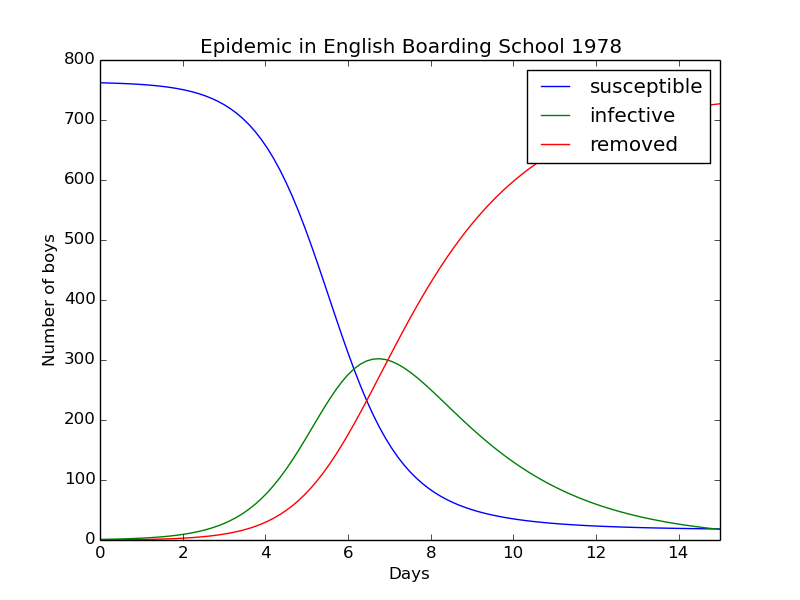
\includegraphics[width=0.9\linewidth]{1_fig/English_boarding_school.png}}
  \caption{
  \label{fig:english_boarding} An English boarding school is modeled for 15 days with the following parameters: $N=763$, $S_0=762$, $I_0=1$, $R_0=0$, $\rho=202$ and $r=2.18 x 10^{-3}$. An increase in the \emph{Infected} group can be seen since $S_0 > \rho$.
  }
\end{figure}
%\clearpage % flush figures fig:english_boarding


\subsection{Maximum concentration of \emph{Infected}}
The maximum concentration of the \emph{Infected} group can be found by usin the threshold value. The result can be compared to the simulation in Fig.(\ref{fig:english_boarding}). Maximum of \emph{Infected} can be found by the following equation from Eq.(\ref{eq:max_I})
\begin{equation} \label{eq:max_I_eng}
\Imax= N - \rho + \rho \ln\frac{\rho}{S_0} 
\end{equation}
By inserting the parameters from the simulation in Fig.(\ref{fig:english_boarding}) in Eq.(\ref{eq:max_I_eng}), the value of $\Imax = 292$. The $\Imax$ of the simulation can be found by checking the maximum number of the infected list. This is similar as the calculated $\Imax$. This maximum value of the \emph{Infeced} group occurs when the $Susceptible$ group is 202, and similar to the value of $\rho$ in the simulation.

\subsection{Variation in parameter value $\rho$}
The parameter value $\rho$ has a major impact on the result. The epidemic disease could turn out quite differently than in the situation in Fig.(\ref{fig:english_boarding}), caused by variations in $a$ and $r$. Fig.(\ref{fig:rho_changes}) consists of some examples where $\rho$ varies from 50 to 400.


\begin{figure}[ht]
  \centerline{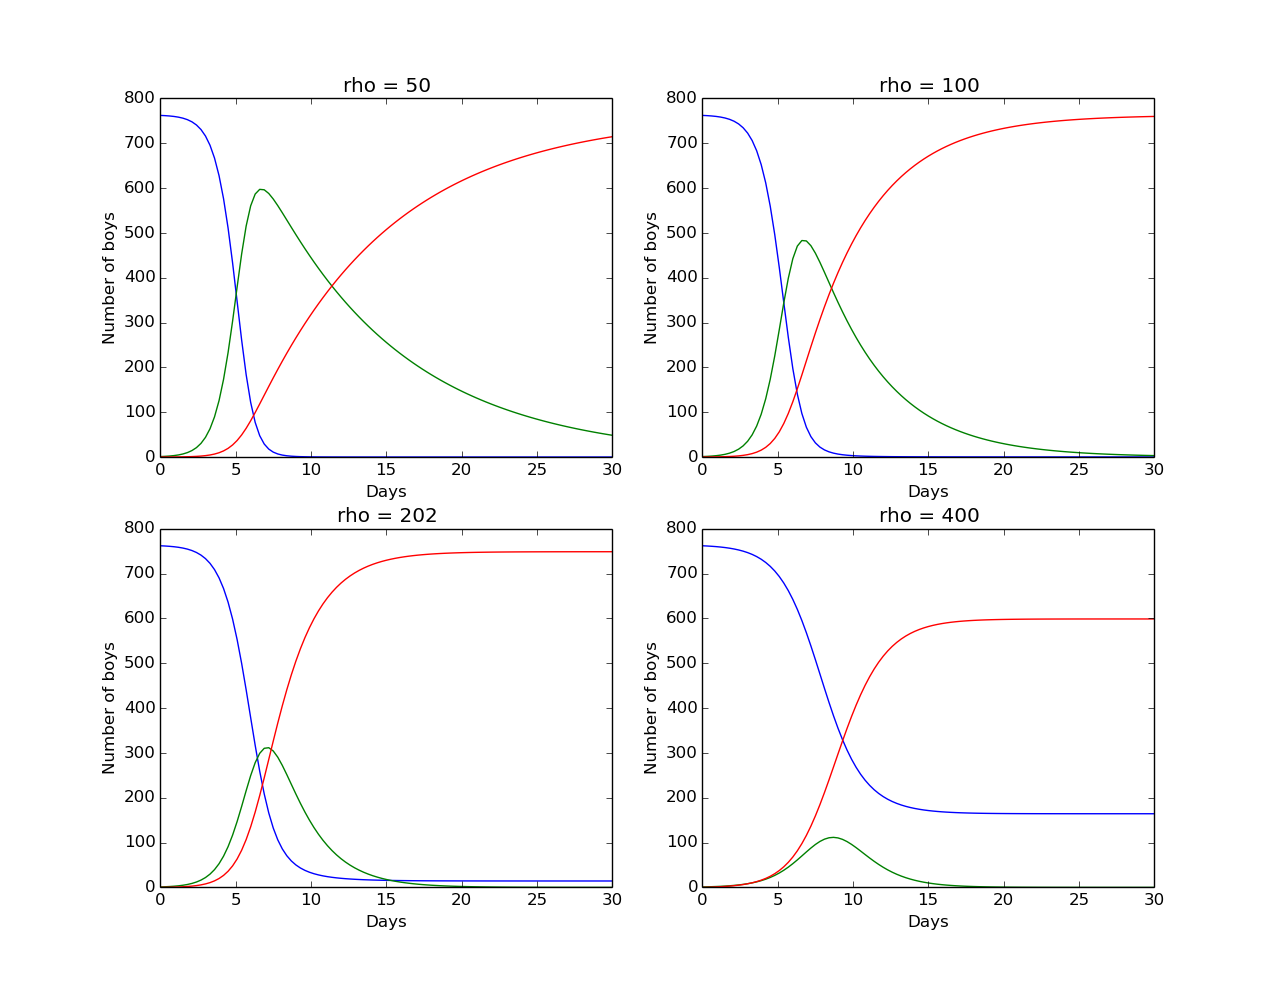
\includegraphics[width=0.9\linewidth]{1_fig/English_boarding_school_changes.png}}
  \caption{
  \label{fig:rho_changes} In the first plot where $\rho=50$, the \emph{Infected} group will increase until the number of \emph{Susceptible} falls down to 50. This will result in a majority of infected students. In the last plot where $\rho=400$, the total number of \emph{Susceptible} stays around 170 students and will go towards a steady number as $I(\infty)=0$.
  }
\end{figure}
%\clearpage % flush figures fig:rho_changes


\section{Zombification}
One of the worst epidemics that can affect the human population is a zombie attack. This will have a huge impact on the way humans live today. Several movies and series has illustrated this type of situation, but it is time that the scientists also take this threat seriously. There have been written a couple of papers about this. Munz et. al\cite{munz2009zombies} used the SEIR model to simulate a possible upcoming zombiefication, where the latent group($E$), is replaced with an \emph{Infected} group($I$) and the \emph{Infected} group($I$) is replaced with a \emph{Zombie} group($Z$). Here it is important to know that the \emph{Infected} group in the $SIZR$ is not the same as in the $SEIR$ model. The following model was used,

\begin{align*}
\frac{dS}{dt} =& \Sigma -\beta SZ - \delta S \\
\frac{dI}{dt} =& \beta SZ - \varrho I - \delta I\\
\frac{dZ}{dt} =& \varrho I + \zeta R - \alpha SZ\\
\frac{dR}{dt} =& \delta S + \delta I + \alpha SZ - \zeta R
\end{align*}

This is a bit more complicated than the standard $SEIR$ model. A presentation of the parameters;
\begin{itemize}
\item $\Sigma$ describes the birthrate for new \emph{Susceptible}. $\frac{dS}{dt}$ is now able to be positive. This is now not a closed system. 

\item $\beta SZ$ describes the numbers of \emph{Susceptible} that become infected , based on interactions between zombies and humans. Similar to the case for $rSI$ in the SIR model. 

\item $\delta$ describes the number of natural deaths in the group. This is used in the \emph{Susceptible} and the \emph{Infected} group

\item $\varrho I$ describes the probability for an infected human to wake up as a zombie.

\item $\zeta R$ controls the number of \emph{Removed} that arises as \emph{Zombie}. 

\item $\alpha SZ$ describes the number of zombies killed by humans in the zombie attacks. 
\end{itemize}

\noindent


\vspace{3mm}




\vspace{3mm}


This model was challenged by Langtangen, Mardal and Røtnes \cite{zombie-math} now referred to as LMR, where they developed another model. They had three objections to the model from Munz et al.~\cite{munz2009zombies}. LMR argue that dead zombies cannot become functioning zombies again. Therefore $\zeta$ will be zero, if magic is not introduced. They let the parameters in the model change with time, according to different phases. LMR argue that the behavior will change with time during a zombie attack. The parameters in the model from LMR was based on the movie \emph{The Night of The Living Dead}. This was done to reproduce its scenarios and then predict how a zombie outbreak would appear. There is also added a function $\omega(t)$, which creates a massive attack from the humans. This is controlled by a time variable and give the \emph{Susceptible} a chance to fight back. The system can be seen in Eq.(\ref{eq:LMR_model}):
\begin{equation} \label{eq:LMR_model}
	\begin{aligned} 
	\frac{dS}{dt} =& \Sigma -\beta SZ - \delta_SS \\
	\frac{dI}{dt} =& \beta SZ - \varrho I - \delta_II\\
	\frac{dZ}{dt} =& \varrho I- (\alpha+\omega(t))SZ + \zeta R\\
	\frac{dR}{dt} =& \delta_SS +\delta_II -\zeta R + (\alpha+\omega(t))SZ 
	\end{aligned}
\end{equation}
The main change is the $\omega(t)$. This is a Gaussian curve and can be seen in eq(\ref{eq:omega}).
\begin{equation} \label{eq:omega}
\omega(t) = a \sum^m_{i=0}\exp\left(\frac{1}{2}\left(\frac{t-T_i}{\sigma}\right)^2\right)
\end{equation}
$\omega(t)$ controls the attacks from the \emph{Susceptible}, which will be fired at predefined time steps. These are controlled by the three parameters. 
\begin{itemize}
\item $a$ here works as a similar parameter as $\alpha$, but will only be activated when the \emph{Susceptible} group is organized and ready to attack. 

\item $T$ contains a list of numbers, which controls the time when the attacks will occur.

\item $\sigma$ controls the length of the attack. 
\end{itemize}

\noindent
This function will be modeled later when it is used in section~\ref{section:counter_attack}


\vspace{3mm}




\vspace{3mm}



\subsection{Parameters used in the model}
The parameter values are essential factors when modelling a zombie attack. Data from the movie \emph{The Night of The Living Dead} was used as basis for the parameters in the ODE system from LMR \cite{zombie-math}. This thesis is based on a thorough study of the TV series \emph{Walking Dead} \cite{walking_dead}. The data will be based on the first five episodes and are constructed after having watched the episodes carefully. The three phases in a zombie attack will be based on the form used in the paper from LMR, but with an extended version in the \emph{Counter attack phase} .

\subsection{The initial phase}
The disease is not yet known in this phase and humans try to save the sick ones by taking them to hospitals or getting some kind of treatment. Because of this ignorance related to the disease, the number in the \emph{Infected} group is high. This phase is often quite short and humans soon start to realise that the risk of getting infected by saving others is really high. \emph{Walking Dead} never shows anything from this phase, but the viewer sees the results when the main character sheriff Rick Grimes wakes up at the local hospital. What he sees is the major damage caused in the initial phase, while the society has moved to the hysterical phase.


\vspace{3mm}




\vspace{3mm}


To determine the values for each group in each phase, the length of Ricks coma is essential. There are several factors that give an indication of the time aspect. When Rick wakes up at the hospital, he has grown a smooth beard of about 1 cm. This would correspond with 1 month in average for a male of European origin. He also has some flowers that have dried out. These also give the impression that some weeks have gone by. The hospital is running on its emergency generator. This would probably not last for many days with a fully operational hospital, but the hospital is as well as shut down when Rick wakes up and can give the emergency generator a longer lifetime. Dr.~Edwin Jenner gives the viewer some information in episode 5 where he tells the videolog that it was 63 days since the epidemic started spreading. By studying the first five episodes in detail, one gets an impression that the time aspect has not been in focus. Therefore the different phases are constructed from the information that has been given. Rick Grimes has probably been in a coma for a month and what he meets the first days will be the basis for the number in each group. The total amount of objects in the model will be based on the number of humans, dead and zombies seen in the first five episodes. 
\begin{itemize}
 \item The number of humans has been estimated to 62. 20 living in the camp with Rick, 40 humans in the old nursing home and the father and son in episode 1. 

 \item The number of dead is estimated to 200. This is based on the amount of dead outside the hospital where Rick woke up. 

 \item The number of zombies are assumed to be 360. These are based on the 30 outside the house of Morgan Jones and his son Duane, 300 zombies in the city Atlanta and 30 zombies attacking the camp. 
\end{itemize}

\noindent
The total number will be 622, and the time aspect aroud a month, which means that these numbers are for the hysterical phase.Over the three first days when Rick is awake, 1 human and 20 zombies are killed in battles. This can be used to find the final number in the initial phase by calculating backwards. By going nine similar periods backwards, the number of killed zombies is 190. The same can be done for humans, which then results in 9 killed humans in this period. The final number for the initial phase can then be set to 71 humans, 540 zombies/infected and 20 dead. This is the same number as for the initial values for the hysterical phase, since the phases are connected.


\vspace{3mm}




\vspace{3mm}


Another issue to discuss is the incubation time. Here there are two examples that can be used. The first transformation from human to zombie happens for the character Amy, who was bit in the arm by a zombie. The transformation happens in about 12 hours. The other example is character Jim who has a slower transformation. This lasts for about two days before the rest of the group leave him alongside the road on their way to CDC(Center for Disease Control). An estimate of the incubation time can be set to 24 hours based on these two transformations.


\vspace{3mm}




\vspace{3mm}


The ODE system in Eq.(\ref{eq:LMR_model})can be used to model the initial phase. The expected results are $S_0 = 621$ and $Z_0 = 1$ while the two other groups are set to zero. The value of $\beta$ can be found with the expression $\beta \Delta t S Z$ from the first ODE equation. After three days about 90 percent of the humans are killed.
\begin{equation}
	\begin{aligned}
	\beta\Delta t S Z &= 0.9 S\\
	3\beta   &= 0.9 \\
	\beta &= 0.3 \\
	\end{aligned}
\end{equation}
The probability of a human being infected will be set to $\beta = 0.3$. The natural death and the birth number is set to 0, since the simulations are performed over short period and for a small group. $\delta_S = \Sigma = 0$. It is quite hard to find similar realistic data for infected humans, so $\delta_I = \delta_S$. Since this is data for the initial phase, zombies are seen as infeteced humans that can be saved. Therefore $\alpha = 0$. And the two last parameters are also zero, $a = \zeta = 0$. The initial phase is modeled in Fig.(\ref{fig:initial_phase_1}):


\begin{figure}[ht]
  \centerline{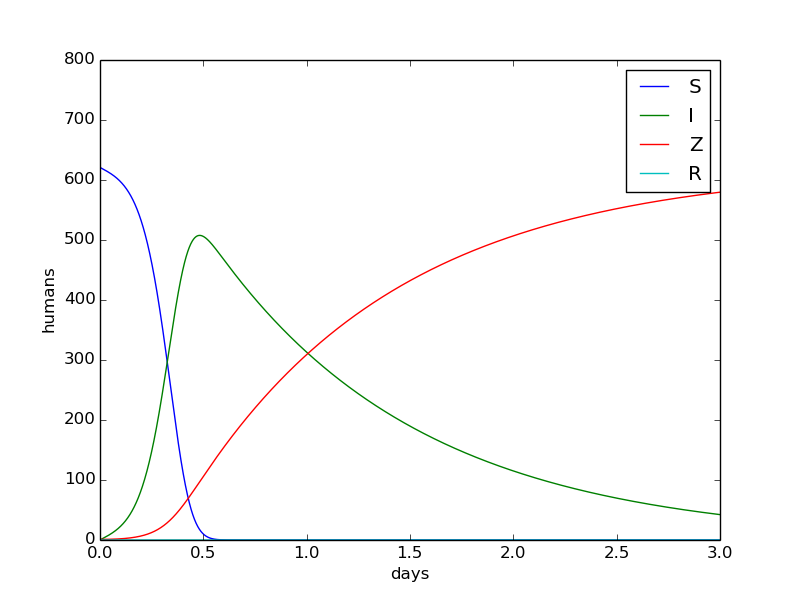
\includegraphics[width=0.9\linewidth]{1_fig/WD_zombie_initial_1.png}}
  \caption{
  \label{fig:initial_phase_1} Initial phase for \emph{Walking Dead}. $\beta=0.3$, $\varrho=1$ and $\alpha=0$ leads to eradication.
  }
\end{figure}
%\clearpage % flush figures fig:initial_phase_1


The result from Fig.(\ref{fig:initial_phase_1}) shows that the human population is eradicated in about a half day. This is not the case, and some adjustments need to be done. There are three parameters that are interesting to study. The first one is $\beta$, which describes how many humans that get infected in a human-zombie collision. The second one is $\varrho$. This parameter controls the incubation time. The last parameter that can affect the number in each group is $\alpha$. This describes the number of zombies killed in a human-zombie collision. These variables are plotted separately and combined in Fig.(\ref{fig:initial_parameters}). The idea here is to produce results that fulfill the final number for the groups \emph{Susceptible} and \emph{Removed} , which is 71 and 20. The blue dot in each plot describes this value. A rough estimate has been done for each parameter before using it. This is why they all lie in different regions than the parameter value in Fig.(\ref{fig:initial_phase_1})



\begin{figure}[ht]
  \centerline{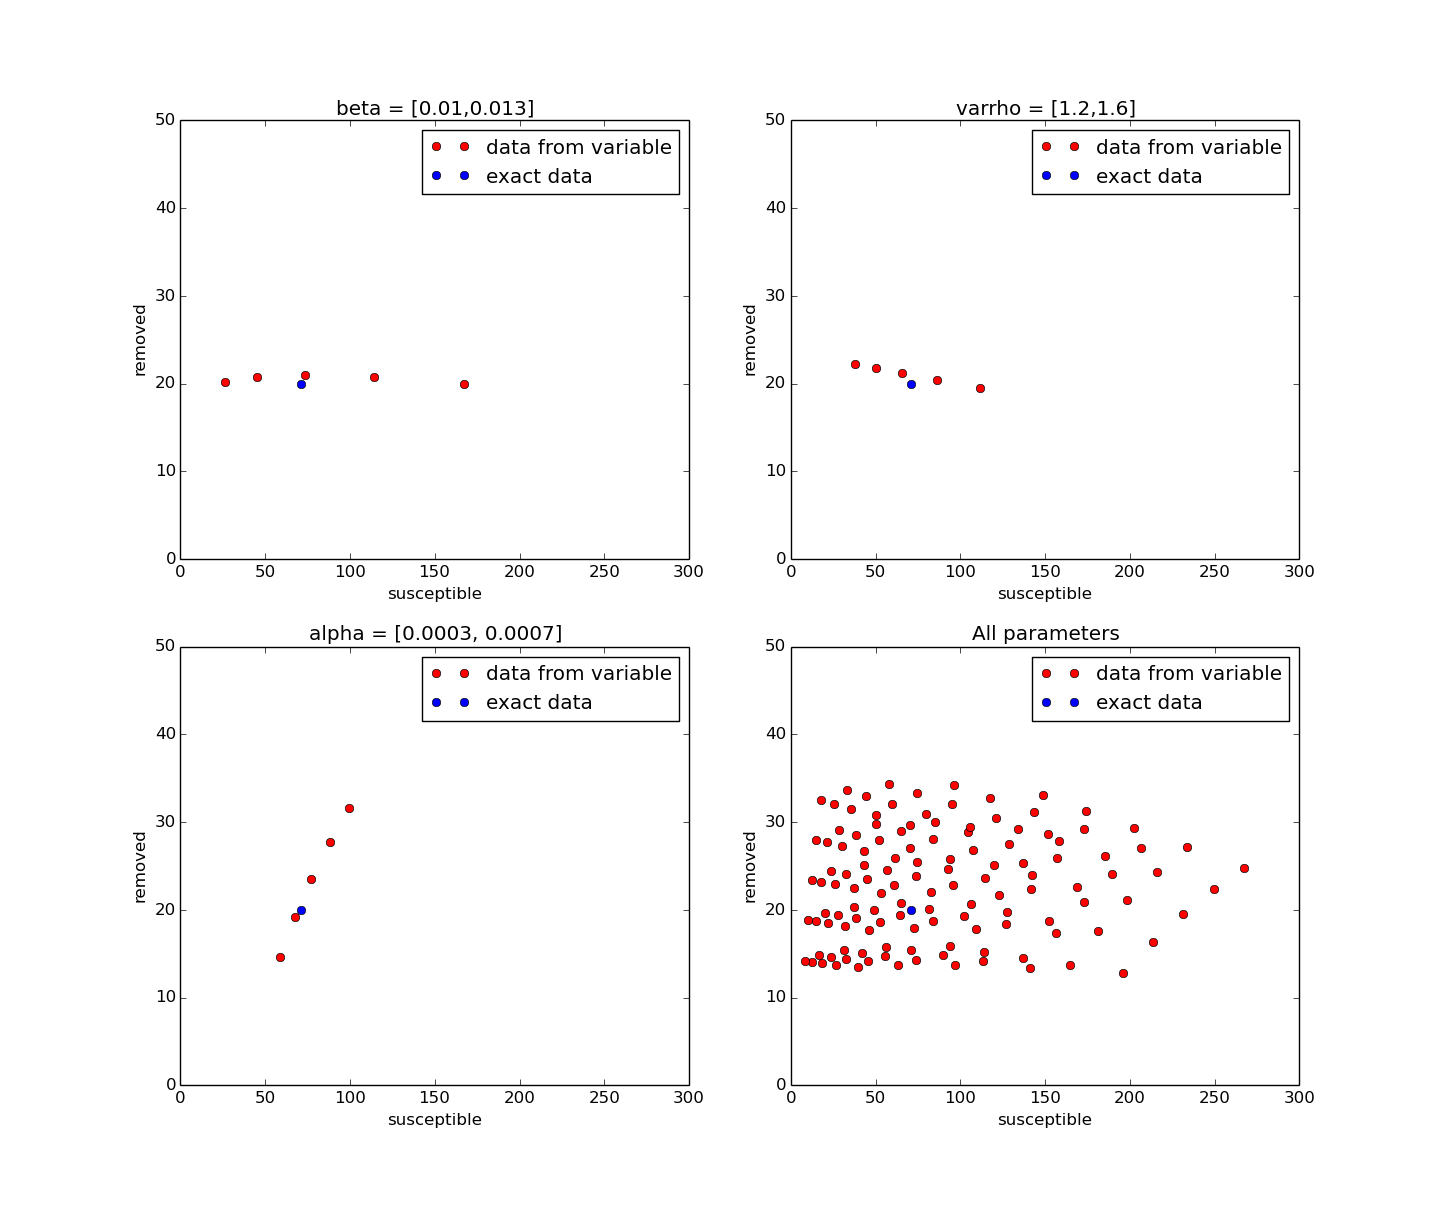
\includegraphics[width=0.9\linewidth]{1_fig/check_parameters.png}}
  \caption{
  \label{fig:initial_parameters} The final result for \emph{Susceptible} and \emph{Removed} group. These plots give a knowledge in the effect of varying the parameters. $\beta$ and $\varrho$ mainly affect the number of \emph{Susceptible} while $\alpha$ affect them both.
  }
\end{figure}
%\clearpage % flush figures fig:initial_parameters


By choosing $\beta = 0.01155$, $\varrho=1.37$ and $\alpha=0.00044$, the following plot can be seen in Fig.(\ref{fig:initial_phase_2}):  


\begin{figure}[ht]
  \centerline{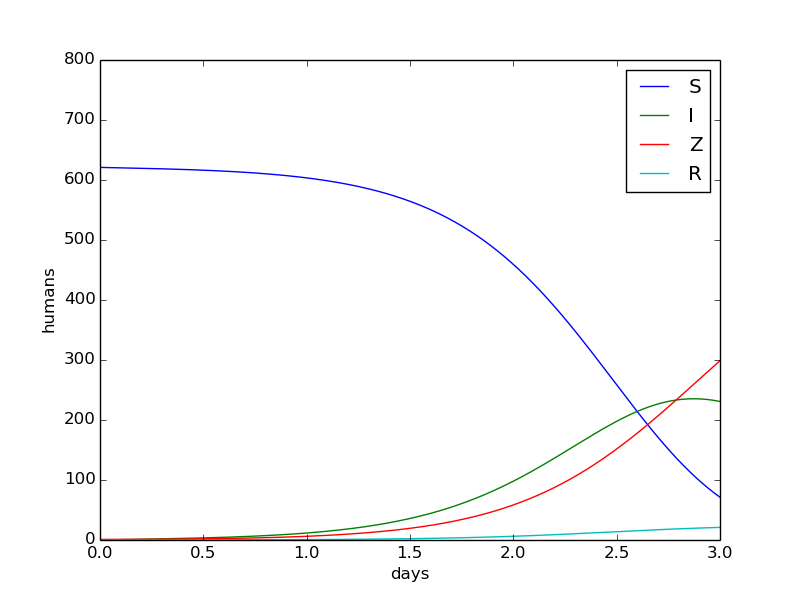
\includegraphics[width=0.9\linewidth]{1_fig/WD_zombie_initial_2.png}}
  \caption{
  \label{fig:initial_phase_2} The final values are $S_n=71.3,I_n=230.8,Z_n=298.9$ and $R_n=21$, which is quite close to the result from the movie.
  }
\end{figure}
%\clearpage % flush figures fig:initial_phase_2


It is possible to argue for the changes done in Fig.(\ref{fig:initial_phase_2}). Increasing $\varrho$ to 1.37 reduces the incubation time. Now the average time will be about 17.5 hours, which is realistic. The probability $\beta$ is sensitive and has a major effect only by small variations. This is due to the term that it is a part of $\Delta t SZ \beta$. A couple of examples demonstrate this. One hour can be estimated by setting $\Delta t = 1/24$. When using the initial values for the groups $S$ and $Z$ and $\beta=0.01155$ from Fig.(\ref{fig:initial_phase_2}). A rough estimate of the \emph{Infected} group in the first hour will be $(1/24)*721*1*0.01155=0.34$. About one-third of a human in the first hour seems as a slow and not very aggressive disease. However when the number of \emph{Zombies} slowly increases, the number of infected will be affected. By looking at the hour when the values are equal between humans and zombies, about 200 in each group, the number of infected will be 19.25 per hour. This result in about 10 percent of the humans. By changing $\beta$ to the value from Fig.(\ref{fig:initial_phase_1}), the number of infected will be 500 per hour and it is quite easy to see that this will lead to eradication in a short amount of time. The last parameter $\alpha$ controls the number of zombies that dies in collisions between zombies and humans. While humans still think that the infected can be saved, it is still a chance that the result from a collision can end with a zombie kill. These results can therefore be seen as realistic values.

\subsection{The hysterical phase}
Now the humans start to avoid the infected and some try to fight them. The humans often gather in groups and try to find safe spots away from the zombies. Important supplies as weapons and food are their main priorities. Barricades are built and the guarding is strict. When Rick Grimes wakes up, the hospital is abandoned and the halls are filled up with dead people. Quite fast he understand that he needs to reach safety. After a couple of days he ends up in a camp outside Atlanta city. A couple of elementary changes has happened with the interaction between humans and infected/zombies. In the initial phase, the humans tried to help the infected humans. This resulted in a high percent of infected. Now they understand this risk and keep distance to those who are infected. This will give $\beta$ a lower value. The morality for a zombie kill has dramatically changed. While this was seen as no option in the initial phase, this is now okay. The humans have started to treat zombies and infected as enemies instead of sick allies. This results in a higher death rate among the zombies, which is described by $\alpha$. 


\vspace{3mm}




\vspace{3mm}


The hysterical model can be constructed based on the data found in the initial phase. 


\begin{quote}
\begin{tabular}{ccc}
\hline
\multicolumn{1}{c}{ hysterical phase } & \multicolumn{1}{c}{ initial values } & \multicolumn{1}{c}{ final values } \\
\hline
S                & 71.3           & 62           \\
I                & 230.8          & -            \\
Z                & 298.9          & 360          \\
R                & 21             & 200          \\
\hline
\end{tabular}
\end{quote}

\noindent
Here, the infected and zombies are counted as one group for the final values, since it is difficult to separate these groups in the series. The time aspect will be modeled for 30 days, which results in a ten times longer simulation. Since the final results are known here, a similar adjustment of the parameters can be done. The range of the parameter values have been found by some test simulations.In Fig.(\ref{fig:hysterical_variations}) the parameters of $\beta$, $\varrho$ and $\alpha$ have been simulated with different values. 


\begin{figure}[ht]
  \centerline{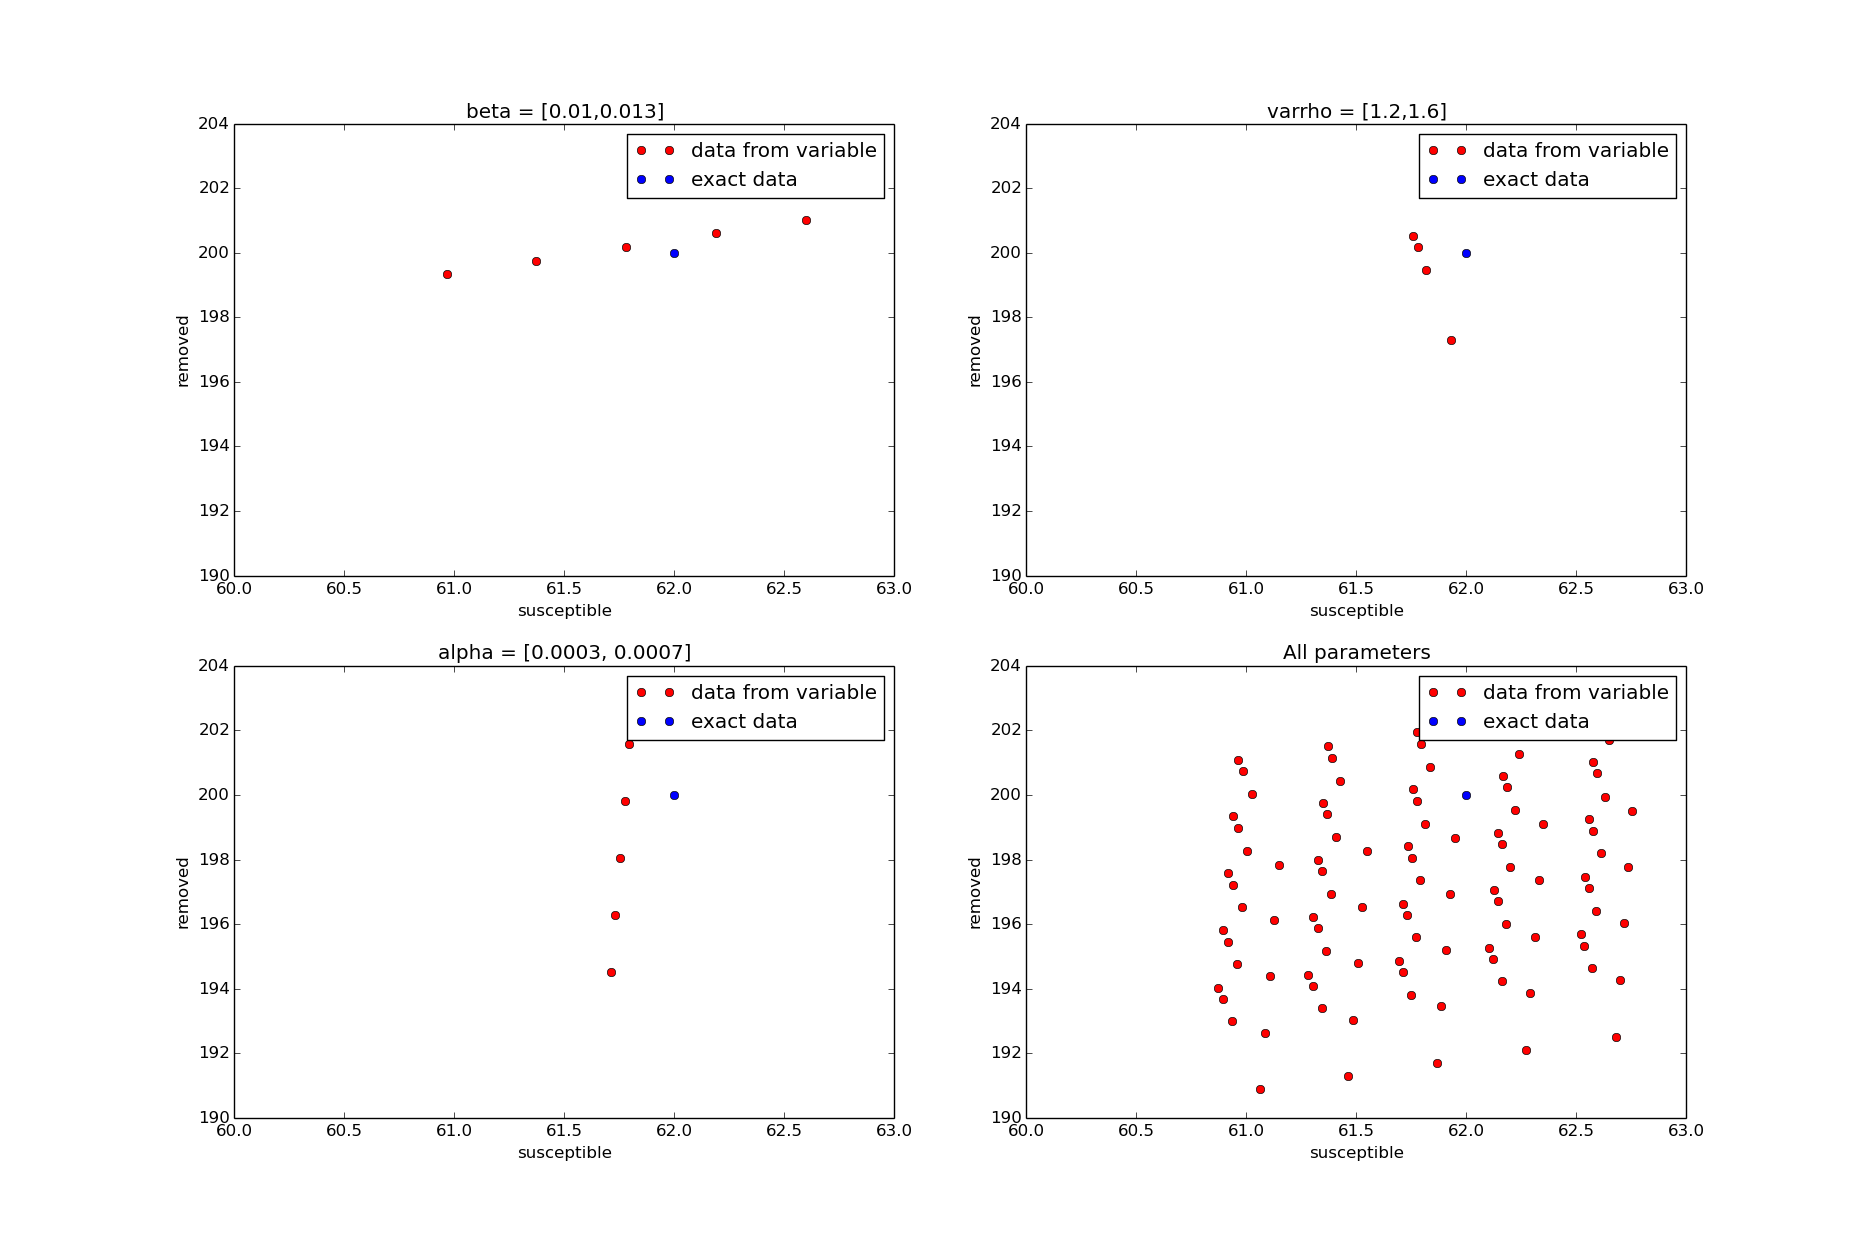
\includegraphics[width=0.9\linewidth]{1_fig/check_parameters_hysterical_2.png}}
  \caption{
  \label{fig:hysterical_variations} Variation in three different parameters in the hysterical phase. The last subplot consist of the combination of all. $\beta=[1\cdot10^{-5},1.2\cdot10^{-5}]$, $\varrho=[1,2]$ and $\alpha=[2\cdot10^{-4},2.2\cdot10^{-4}]$
  }
\end{figure}
%\clearpage % flush figures fig:hysterical_variations


Fig.(\ref{fig:hysterical_variations}) gives insight in how variations in parameters affect the final result. By decreasing $\beta$, it will essentially increase the number of \emph{Susceptible} that will survive, but it will also increase the number of deaths. This may at a first glance seem quite strange. Should not the number of deaths decrease when the number of surviving humans increase? This can be explained with the idea that was shown for $\beta$ in the initial phase. Since $\beta SZ$ gets smaller when $\beta$ gets smaller, the combination of $SZ$ will stay higher for a longer time . This will again affect $\alpha SZ$, which regulates the number of killed zombies. The larger this combination is, the more zombies will die. 


\vspace{3mm}




\vspace{3mm}


By increasing $\alpha$, the number of \emph{Removed} also increase. However similar to the increasing of the \emph{Removed} it also has a slight increase on the number of \emph{Susceptible}. Here the argument for $\beta$ above can be reversed. Since a higher $\alpha$ leads to a higher death rate among the zombies, the combination $SZ$ will be smaller, which makes $\beta SZ$ smaller.


\vspace{3mm}




\vspace{3mm}


The last parameter, $\varrho$, has nearly no effect. The red dots show a small decreasing of \emph{Removed} and increasing of \emph{Susceptible}  when $\varrho$ is increased. This parameter varies most, but has least impact. This can be explained with the long time aspect and the low number of infected compared to the number of zombies. Since the number of zombies is much higher, the transformation length from infected to zombie is almost negligible.  


\begin{figure}[ht]
  \centerline{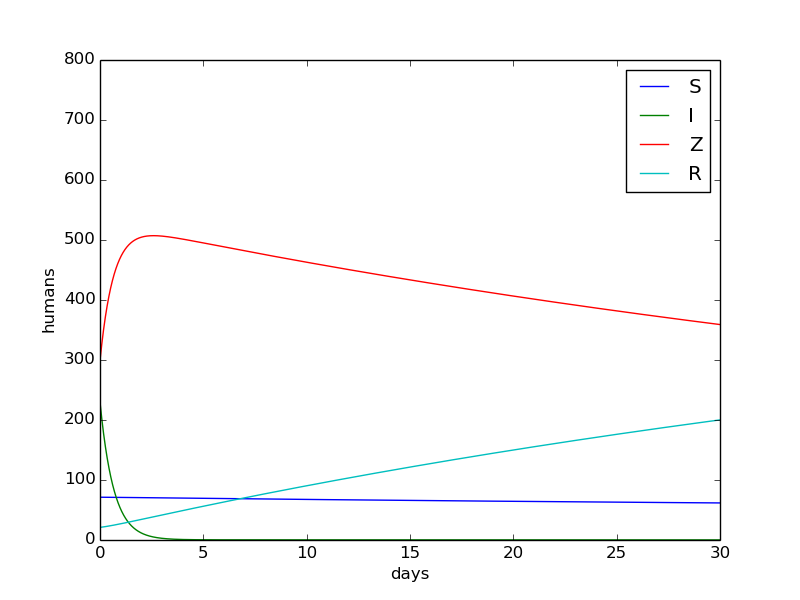
\includegraphics[width=0.9\linewidth]{1_fig/WD_zombie_hysterical_1.png}}
  \caption{
  \label{fig:hysterical_1} Hysterical phase with parameter values $\beta = 0.000011$, $\varrho = 1.5$ and $\alpha = 0.000208$.
  }
\end{figure}
%\clearpage % flush figures fig:hysterical_1


Fig.(\ref{fig:hysterical_1}) fulfills the result that was predicted based on the series. These final numbers correspond with the number in each group when Rick woke up at the hospital. The plot shows that the number of zombies increases quickly and reaches its maximum value after a couple of days in this phase, similar to the number of infected that dramatically decreased. Here the humans have been able to stabilize. Since the clashes between humans and zombies are dramatically decreased, nearly no humans get infected. And in the cases where humans have to face zombies, the killing rate has increased. The increase of \emph{Removed} is close to proportional to the decrease of \emph{Zombies}, which means that it is mostly zombies that die.

\subsection{The counter attack}
\label{section:counter_attack}
This counter attack is more complicated to model, since this phase appears simultaneously as the hysterical phase in \emph{Walking Dead}. The group of humans are trying to avoid the zombies, but when the zombies get too close, the humans need to fight back. These situations are caused by a high density of zombies in some areas, which force the zombies to spread. In \emph{Walking dead} the counter attack appears when a group of 30 zombies reach the camp. This triggers a fight where all the zombies are killed and 4 of the humans get bitten. This shows that a counter attack from the humans causes a lot of damage. The time aspect is set to 6 hours.  


\vspace{3mm}




\vspace{3mm}


Now the function $\omega(t)$ will be used. This can be seen in Fig.(\ref{fig:omega_function}):


\begin{figure}[ht]
  \centerline{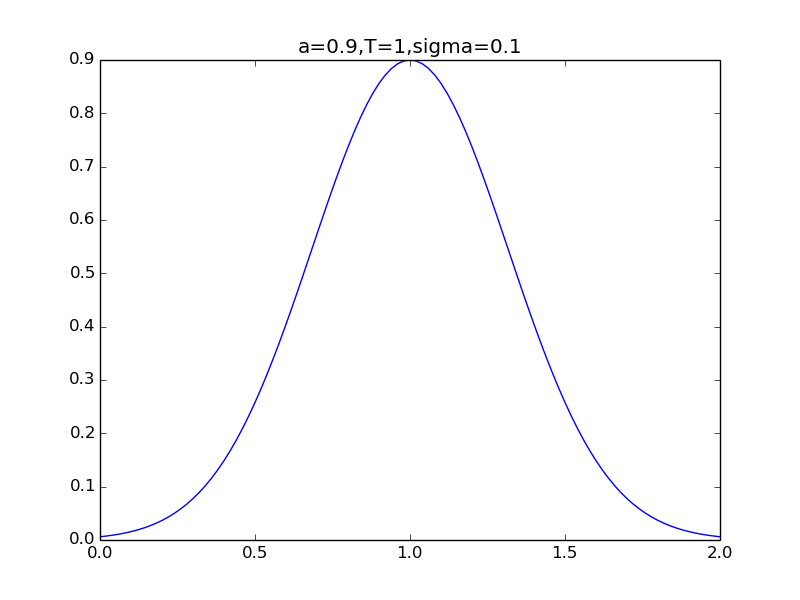
\includegraphics[width=0.9\linewidth]{1_fig/omega_function.png}}
  \caption{
  \label{fig:omega_function} $\omega (t)$ is a Gaussian function where $a$ controls the maximum value, $T$ controls the time for maximum value and $\sigma$ controls the length of the attack.
  }
\end{figure}
%\clearpage % flush figures fig:omega_function


To get some start values, $SZ\omega(t)=30$ can be used. Where $\omega(t)$ is the area under the function. By inserting the final values from hysterical phase for $S$ and $Z$, the area shall be $\omega (t)=1.34\cdot10^{-3}$. This result can be reproduced by using $a= 0.00103$ and $\sigma = 0.005$ in $\omega(t)$. The counter attack is sat to appear during the last part of the day [0.75,1]. The value of T is then set to $T$=[0.875].


\begin{figure}[ht]
  \centerline{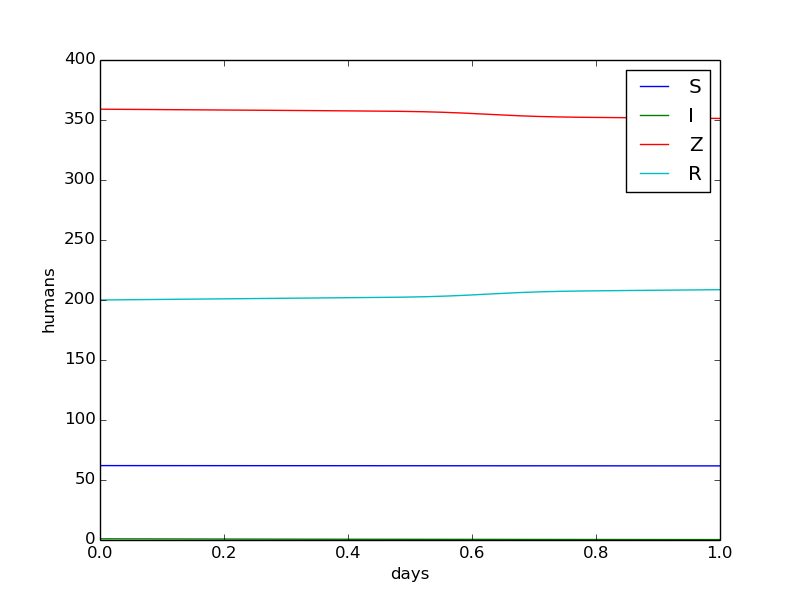
\includegraphics[width=0.9\linewidth]{1_fig/WD_zombie_counter_1.png}}
  \caption{
  \label{fig:zombie_counter_1} The counter attack. 8-9 zombies are killed and all humans survive
  }
\end{figure}
%\clearpage % flush figures fig:zombie_counter_1


This simulation in Fig.(\ref{fig:zombie_counter_1}) results in some deaths. However, the total number should be higher. Another problem is that no humans died during this battle. The ODE model (\ref{eq:LMR_model}) is based on \emph{The Night of the Living Dead}, where the amount of humans who are killed is close to zero. This is not the case in \emph{Walking dead}. Therefore the risk of dying is higher for human during a counter attack. This is solved by adding $\mu \omega (t) SZ$, where $\mu$ is the risk for a human getting infected compared to a zombie kill during this attack. The model (\ref{eq:LMR_model}) can then be expanded to system(\ref{eq:1_seland_model}),

\begin{equation} \label{eq:1_seland_model}
	\begin{aligned} 
	\frac{dS}{dt} &= \Sigma -(\beta+\mu \omega(t))SZ - \delta_SS \\
	\frac{dI}{dt} &= (\beta+\mu \omega(t))SZ - \varrho I - \delta_II\\
	\frac{dZ}{dt} &= \varrho I- (\alpha+\omega(t))SZ + \zeta R\\
	\frac{dR}{dt} &= \delta_SS +\delta_II -\zeta R + (\alpha+\omega(t))SZ 
	\end{aligned}
\end{equation}


\begin{figure}[ht]
  \centerline{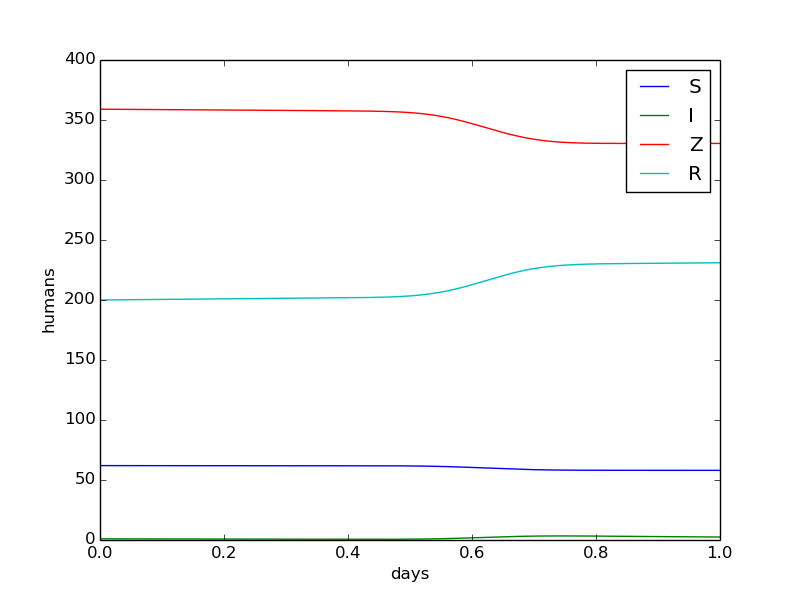
\includegraphics[width=0.9\linewidth]{1_fig/WD_zombie_counter_2.png}}
  \caption{
  \label{fig:zombie_counter_2} Counter attack with the new model. Parameter values are set to $a=0.0073$ and $\mu=0.14$.
  }
\end{figure}
%\clearpage % flush figures fig:zombie_counter_2


Fig.(\ref{fig:zombie_counter_2}) is modeled with the initial values given when Rich woke up, explained in the initial phase. The result after this day is that the humans are reduced to 58 humans. The number in the \emph{Infected} group is increased to 2.47, which can be explained with the two characters in the series, Amy and Jim. The number of \emph{Removed} is increased to 231, and is a combination of killed zombies and humans who are attacked. By modelling this for another day, the \emph{Removed} group will increase with a couple of new deaths. 


\vspace{3mm}




\vspace{3mm}


It would be interesting to check what would happen if this counter attack was repeated over time. Who would survive? An attack every other day will give the following result shown in Fig.(\ref{fig:counter_series})


\begin{figure}[ht]
  \centerline{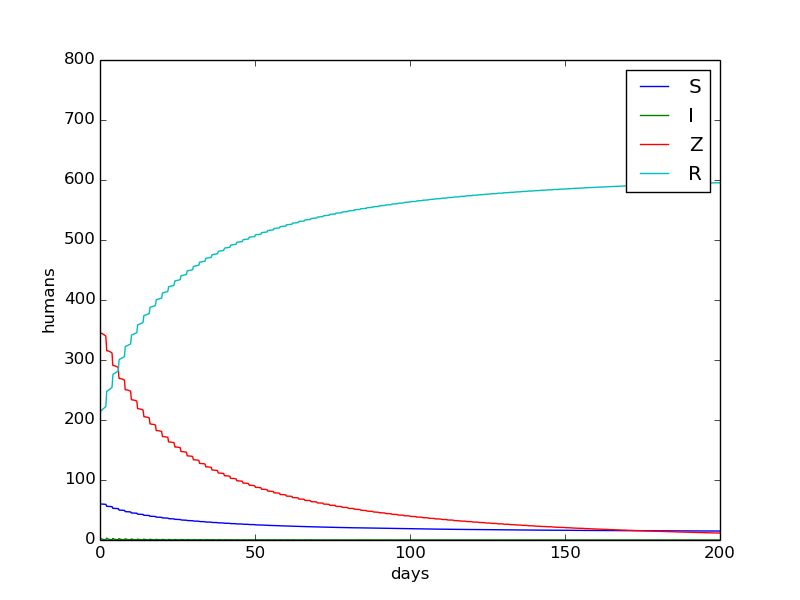
\includegraphics[width=0.9\linewidth]{1_fig/WD_zombie_counter_series.png}}
  \caption{
  \label{fig:counter_series} 100 counter attacks during 200 days will result in a higher population of humans.
  }
\end{figure}
%\clearpage % flush figures fig:counter_series


After 200 days there would be about 15 humans and 12 zombies left. Then the humans would be able to survive since they are more efficient in battles. 

\subsection{The three phases in Walking Dead}
By adding these three phases together, the final result after the attack should be possible to match. The simulation here will be done with the parameters used in the earlier sections. This can lead to a small error since the result of the final number in each phase is given with decimals and the initial values are based on assumptions and round off numbers. The different parameter values are listed in Tab.(\ref{table:param_val}). 

\label{table:param_val}

\begin{quote}
\begin{tabular}{cccc}
\hline
\multicolumn{1}{c}{ parameter } & \multicolumn{1}{c}{ Initial phase } & \multicolumn{1}{c}{ hysterical phase } & \multicolumn{1}{c}{ counter attack } \\
\hline
$\beta$   & 0.01155       & 0.000011         & 0.00011        \\
$\varrho$ & 1.37          & 1.5              & 1.5            \\
$\alpha$  & 0.00044       & 0.000208         & 0.000208       \\
a         & 0             & 0                & 0.0073         \\
$\sigma$  & 0             & 0                & 0.005          \\
$\mu$     & 0             & 0                & 0.14           \\
\hline
\end{tabular}
\end{quote}

\noindent
The simulation is run for 34 days. The three first days are in the initial phase, the resisting days are in the hysterical phase. The counter attack is released on day 33 and lasts for about 6 hours. The plot is shown in Fig.(\ref{fig:all_phases})   


\begin{figure}[ht]
  \centerline{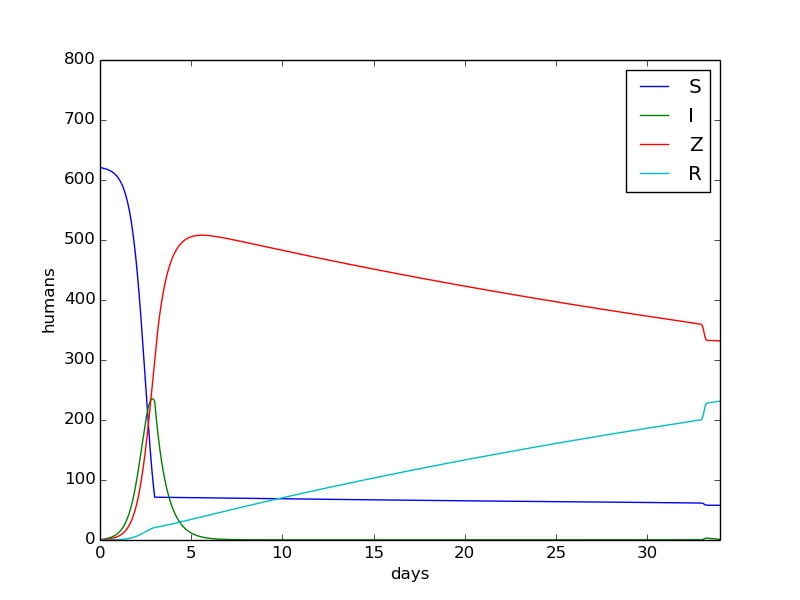
\includegraphics[width=0.9\linewidth]{1_fig/WD_zombie_all_phases_1.png}}
  \caption{
  \label{fig:all_phases} Walking Dead simulated after 5 episodes. Based on the three different phases.
  }
\end{figure}
%\clearpage % flush figures fig:all_phases


Fig.(\ref{fig:all_phases}) clearly shows that the change in parameter values affect the different phases. The different values are shown in the Tab.(\ref{table:group_values}), where the values are given at the initial time. The last column consist of the final values after 34 days.

\label{table:group_values}

\begin{quote}
\begin{tabular}{ccccc}
\hline
\multicolumn{1}{c}{ values } & \multicolumn{1}{c}{ Initial phase } & \multicolumn{1}{c}{ hysterical phase } & \multicolumn{1}{c}{ counter attack } & \multicolumn{1}{c}{ final values } \\
\hline
$S_0$  & 621           & 71               & 62             & 58           \\
$I_0$  & 0             & 231              & 0              & 1            \\
$Z_0$  & 1             & 299              & 359            & 332          \\
$R_0$  & 0             & 21               & 202            & 231          \\
\hline
\end{tabular}
\end{quote}

\noindent
Considering the uncertainty of the parameters, this simulation gives a result close to the expected result. 


\vspace{3mm}




\vspace{3mm}



\section{Discussion}
Two different ODE models are used in this chapter. The first model is a basic SIR model, and the disease in the \emph{English boarding school} is based on this model. The expected result was produced. With variations in the value of $\rho$, it caused large differences in the result for the simulation.


\vspace{3mm}




\vspace{3mm}


The \emph{Zombiefication} part was based on the model and phases from LMR Ref.(\cite{zombie-math}). The parameters and the lenght of the phases were adjusted to simulate \emph{Walking Dead}. Several assumptions were made from the writer to model this series. Since the simulations were based on expected results, the parameters were adjusted to fulfill these demands. The model was able to produce the expected result for the groups, and one can say that the spread can be seen as possible based on these assumptions.    


\vspace{3mm}




\vspace{3mm}


There are several factors that this model don't take into account. How will the number of battles effect the humans and zombies? Will they be tired or more efficient? What about weapons? What would happen if the group of zombies was much larger? Due to different variations in behavior of humans and zombies, one can never predict all situations accurately. This is a weakness with this model, and human behavior is difficult to add to the model.  


\vspace{3mm}




\vspace{3mm}


The parameters found in this model will be used for all three chapters.This model is straight forward to calculate and is easy to use.The model is good if the goal is to find the total amount of each group measured over an area. It demands that the parameters are given. The model gives no information about the spatial spread of the disease. This will therefore be useless in describing how a disease can spread abroad countries and borderlines, or the spatial differences of being infected. The two next chapters will introduce more complicated models which will take the spatial position into account. 



\clearemptydoublepage
\markboth{Bibliography}{Bibliography}
\thispagestyle{empty}

\bibliographystyle{plain}
\bibliography{../bibliography/papers}



% ------------------- end of main content ---------------


% #ifdef PREAMBLE
\clearemptydoublepage
\markboth{Index}{Index}
\thispagestyle{empty}
\printindex

\end{document}
% #endif

